% TODO pas sur mais ca peux etre sympa si on se focus plus a cheerios que ceci est pour un cours peut etre ? je sais pas ? qui sais ? pas moi en tot cas. 
Nous avons tous mangé des céréales ou vu des objets flottant s'attirer ou se repousser entre eux, mais quel est la raison de cette force ? Nous avons essayé de décrire ces interactions dans ce projet.

\begin{table}
    \centering
    \begin{tabular}{ccc}
        \hline
        Nom                & Abréviation & Dimension\\
        \hline
        Rayon de courbure  & $R$         & [$L$]\\
        Surface de tension & $\gamma$    & [$MT^{-2}$]\\ 
        Densité du solide  & $\rho_s$    & [$ML^{-3}$]\\
        Densité du liquide & $\rho_l$    & [$ML^{-3}$]\\
        Densité de l'air   & $\rho_a$    & [$ML^{-3}$]\\
        Nombre de Bond     & $B$         & $1$\\
        \hline
    \end{tabular}
    \caption{Table des variables}
\end{table}

\subsection{Effet Cheerios}
%Ce que Baptiste avait écrit
    \paragraph*{}{
        Cette partie est plutôt faite pour l'intégrité du rapport. Le lecteur est fortement encouragé à lire "Cheerios Effect"\cite{vella_cheerios_2005} pour avoir une compréhension plus complète du sujet. Les calculs viennent principalement de cet article.
    }
    \paragraph*{}{
        Lorsque nous posons un objet sur la surface de l'eau (une aiguille, une punaise ou un cheerio), il est possible que l'objet reste à la surface de l'eau. L'eau va donc se courber, enveloppant une partie de l'objet, sous la masse de celui-ci. Cela se nomme la déformation interfaciale. Elle se retrouve dans la nature avec certains insectes pouvant marcher sur l'eau grâce à cette loi physique. Si nous mettons plusieurs objets de la sorte et qu'ils sont plus ou moins proche, la courbure de l'eau sous ces objets va créer une tension de surface qui attirera les objets jusqu'à qu'ils se touchent. De plus, si nous mettons ces objets dans un récipient, au fil du temps ils vont s'approcher des bords. Nous pouvons également expliquer cela par la tension de surface qui est créée entre le récipient et l'eau qui créera un ménisque.
        }
        
        \paragraph*{}{
            Nous voulons déterminer comment ces objets réagissent entre eux et les bords d'un récipient et représenter nos résultats de façon numérique et animée. Nous devons, pour cela, calculer tout d'abord les forces intervenant dans ce phénomène.
            } 

    %Ce que Erdi a écrit
    TODO expliquer de ou viens les forces des angles qui tord la surface ?

    \begin{figure}[!htb]
        \centering
        \includegraphics[width=0.5\textwidth]{schema_cheerios_objet_eau.tikz}
        \caption{Schéma d'un seul objet proche d'une parois, avec la définition de contact d'angle.}
        \label{objet_seul}
    \end{figure}

    Expliquer leffet de cheerios.
    
    % TODO peut etre notre propre figure ?
    % \begin{figure}
    %     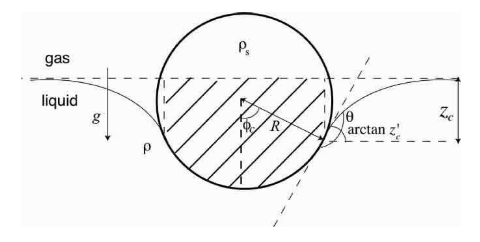
\includegraphics[width = 0.9\textwidth]{boulleflotantedecheerios.png}
    %     \caption{Geometry of a sphere lying at a liquid-gas interface. The shaded area represents the weight of liquid equivalent to the buoyancy force due to hydrostatic pressure acting on the sphere.\cite{vella_cheerios_2005}}
    % \end{figure}
    \begin{figure}[!htb]
        \centering
        \includegraphics[]{schema_geom_sphere_eau.tikz}
        \caption{Géométrie d'une sphère reposant sur une interface liquide-gaz. La partie rayée représente le poids de liquide équivalent à la force de flottabilité du à la pression hydrostatique appuyant sur la sphère. }
        \label{geom_sphere}
    \end{figure}
    % Une des raisons la quel les objets flotte cest due a la pusee de archimede et ces't un des cas majeurs dans notre probleme aussi. Comme on peux voir dans la figure TODO metre la citation de la figure en haut.
    Une des raisons pour laquelle les objets flottent est due à la poussée d'Archimède, comme nous pouvons le voir dans la figure \ref{objet_seul} ou \ref{geom_sphere}. Faut que tu me dises laquelle.
    
    % Pour que notre sphere reste sur linterface il a besoin que son poids \(\frac{4}{3}\pi\rho_{s}gR^3\) devrait etre en equilibre par la composante de pousee de archimede a lendroit de contact du liquide avec la sphere et la force de tension sur la surface ??? must be balanced by the component of surface tension acting along the (circular) contact line and the buoyancy force because of the displaced bulk fluid.
    Pour que notre sphère reste sur l'interface liquide-gaz elle a besoin que la norme de son poids \(||\vb*{P}||=\frac{4}{3}\pi\rho_{s}gR^3\); doit être équilibrée par la composante de tension superficielle agissant le long de la ligne de contact (circulaire) et par la force de flottabilité due au déplacement du fluide en vrac. La première composante a pour équation :
    \begin{equation}
        2\pi\gamma R\sin{\phi_c}\frac{z_c'}{\sqrt{1+z_c^{'2}}}
    \end{equation}

    Et nous avons également la force de flottabilité par l'équation :
    \begin{equation}
        \pi\rho_l g R^3 (\frac{z_c}{R}\sin^2{\phi_c} + \frac{2}{3}-\cos{\phi_c}+\frac{1}{3}\cos^3{\phi_c})
        \label{eq:buoyancyForce}
    \end{equation}

    % TODO expiquer dou ca viens moi ja pas comprie
    % \begin{equation}
    %     2\pi R \phi_c \gamma \sin(\arctan z_c^{'}) = 2\pi\gamma R \sin\phi_c z_c^{'}(1+z_c^{'2})^{-1/2}
    %     \label{eq:wut}
    % \end{equation}

    Nous avons donc l'équilibre des forces donné par :
    \begin{equation}
        \frac{4}{3}\pi\rho_{s}gR^3 =2\pi\gamma R \sin\phi_c \frac{z_c^{'}}{\sqrt{(1+z_c^{'2})}} + \pi\rho_l g R^3 (\frac{z_c}{R}\sin^2 \phi_c + \frac{2}{3}-\cos\phi_c+\frac{1}{3}\cos^3 \phi_c)
    \end{equation}

    % TODO cest quoi $z_c^{'}$??? Un point de contact apparemment 

    Si nous substituons \(\phi_c = \pi - \theta + \arctan z_c^{'}\) et gardons uniquement les termes linéaires en \(z_c^{'}\), nous retrouvons l'expression pour \(z_c^{'}\sin \phi_c\) qui est précis par rapport \textit{à l'ordre linéaire du nombre de Bond}, \(B \equiv R^2/L_c^2\) 

    Nous avons donc:
    \begin{equation}
        z_c^{'}\sin \phi_c = B(\frac{2D-1}{3}-\frac{1}{2}\cos \theta + \frac{1}{6} \cos^3 \theta) \equiv B\Sigma
        \label{eq:bondsigma}
    \end{equation}
    Avec \(D \equiv \frac{\rho_s}{\rho}\).
    
    % On peux voir ceci est bien le cas car on observe bien que \(z_c^{'} = 0\) quand \(\theta = \pi/2\) et \(D = 1/2\) cest ce que on satendais car dans ce cas la pousee de archimede seul lui meme est assez pour equilibrer le poids de la sphere sans deformations du liquide.

    L'équation [\ref{eq:bondsigma}] contient deux paramètres sans dimensions; \textit{le nombre de Bond}$B$ et $\Sigma$, qui sont très importants pour notre modélisation.

    Le nombre de Bond vaut:
    \begin{equation}
        B = \frac{(\rho_l-\rho_{a})gR^2}{\gamma}
    \end{equation}
    Il nous donne la mesure relative de l'importance des effets de gravité et de la tension de surface; si $B$ est tres grand, cela correspond à des particules grandes ou à une tension de surface petite. 

    WUT ????

    The expression for the slope of the interface in the vicinity of the spherical particle given in (9) is valid for B << 1 (corresponding to a radius of  1mm or smaller for a sphere at an air-water interface) in which case surface tension is very important. The other dimensionless parameter, , can be thought of as a (non-dimensional) resultant weight of the particle once the Archimedes upthrust has been subtracted out. This physical interpretation arises naturally from the vertical force balance condition (8) and (9) since the resultant weight of the object (in the linearised approximation) is simply 

    To calculate the interaction energy using the Nicolson
    approximation, we must also calculate the interfacial displacement caused by an isolated floating sphere, which is determined by the hydrostatic balance gamma nabla²h = rho gh - the co-ordinate invariant statement of equation (1). With the assumption of cylindrical symmetry, this becomes:
    \(\gamma \nabla^2h = \rho_l g h\)
    \begin{equation}
        \gamma \frac{\dd^2h}{\dd x^2} = \rho_l g h
    \end{equation}
    Si on assume une symetrie spherique
    \begin{equation}
        \Rightarrow \frac{1}{r} \frac{\dd}{\dd r} \left( r\frac{\dd h}{\dd r}\right) = \frac{h}{L_c^2}
    \end{equation}
    TODO developer bessel
    \cite{introtoBessel}

    % TODO dans le code ajouter un buoyancy force qui calcule la ousee de archimede et dis si notre objet flotte ou pas si il flotte pas on peux metre un option tel quel il prend la valeur automatique ??? Ou on le neglige ????
    % TODO On mets les formules et peut etre demontrer ou ils viennent et surtout les cas ou on peux utiliser ces formules les cas ou ca marche pas etc\ldots
    % TODO SCHEMA deux cheeios et sur le schema on monre l Rayon de courbure etc...
    % TODO graphique des foncions de bessel
    % TODO citer cheerios 
    \begin{equation}
        \label{ForceEntreCheerios}
        F(l) = -2\pi \gamma R B^{5/2} K_1 \left( \frac{l}{L_c}\right)
    \end{equation}
